\documentclass[sigconf,nonacm]{acmart}
\usepackage{booktabs,array,tabularx,tikz,amsmath,pgfplots}
\usepgfplotslibrary{groupplots}
\pgfplotsset{compat=1.18}
\usetikzlibrary{arrows.meta,positioning}
\definecolor{navy}{HTML}{112B45}
\definecolor{blue}{HTML}{1E78B4}
\definecolor{green}{HTML}{167C63}
\definecolor{pale}{HTML}{EAF4F8}
\setlength{\textfloatsep}{8pt plus 2pt minus 2pt}
\setlength{\floatsep}{7pt plus 2pt minus 2pt}
\setlength{\intextsep}{7pt plus 2pt minus 2pt}
\setlength{\emergencystretch}{1em}
\renewcommand{\arraystretch}{1.08}
\settopmatter{printacmref=false,printfolios=true}
\setcopyright{none}
\renewcommand\footnotetextcopyrightpermission[1]{}
\newcommand{\callout}[1]{\par\vspace{4pt}\noindent\colorbox{pale}{\parbox{\dimexpr\linewidth-2\fboxsep\relax}{\small #1}}\par\vspace{4pt}}
\title{Horizon: Evidence-Conditioned Runtime Assurance for Autonomous Maritime Systems}
\author{Tan Wee Joe}
\affiliation{\institution{University College London}\city{London}\country{United Kingdom}}
\email{tanweejoe@gmail.com}
\begin{document}
\begin{abstract}
Horizon separates three questions: is a proposed vessel command physically recoverable, is it supported by current operating-policy evidence, and is the camera model processing its input normally? We implement these functions as an evidence-conditioned physical governor (A5), a gate-owned policy authorization layer (A6), and a temporal sparse perception monitor (H5). This paper combines their controller, perception, GPU, and fault-injection experiments.

In a 60-branch controller study, A5 achieved 99.83\% gate acceptance, with zero collisions in the 45 declared-recoverable branches across all candidates. On 10,110 matched perception records, H5 detected 7 of 33 missed-obstacle proxy events: 21.21\% recall, 59.65\% balanced accuracy, and 0.712 AUROC. A separate repeat-image guard raised sustained-freeze warning coverage from 0/20 to 18/20 fault frames. NVIDIA L4 execution of a 296-frame sequence achieved a 34.91\,ms median instrumented forward pass; including the recorded CPU postprocessing stages raised the median subtotal to 144.75\,ms.

We choose A6 with H5 as complementary policy and perception checks around A5, demonstrating command vetoes, fault warnings, and bounded simulation responses.

\par\smallskip\noindent\textbf{Project repository:} \url{https://github.com/w3joe/horizon}
\end{abstract}
\ccsdesc[500]{Computer systems organization~Robotic autonomy}
\ccsdesc[300]{Computing methodologies~Computer vision}
\keywords{runtime assurance, maritime autonomy, perception health, sparse autoencoders, GPU latency}
\maketitle
\section{Safety objective and system architecture}

A plausible video mask or a confident AI command is insufficient evidence that a vessel should execute that command. The camera may freeze, the model may omit an obstacle, a contact track may be stale, or a proposed maneuver may conflict with the configured operating policy. Horizon separates these questions so that a single model output does not decide its own acceptability.

The external AI proposes a heading and speed. A separate physical governor evaluates recoverability; an independent authorization layer checks the operating policy. A video-model monitor supplies diagnostic warnings. We assign the project code names \textbf{A5}, \textbf{A6}, and \textbf{H5} to these functions, respectively; the numbers identify designs within the assurance and health families. Only the actuator gate dispatches commands. It rechecks evidence and deadlines, while a watchdog retains recovery authority.


\begin{figure}[t]
\centering
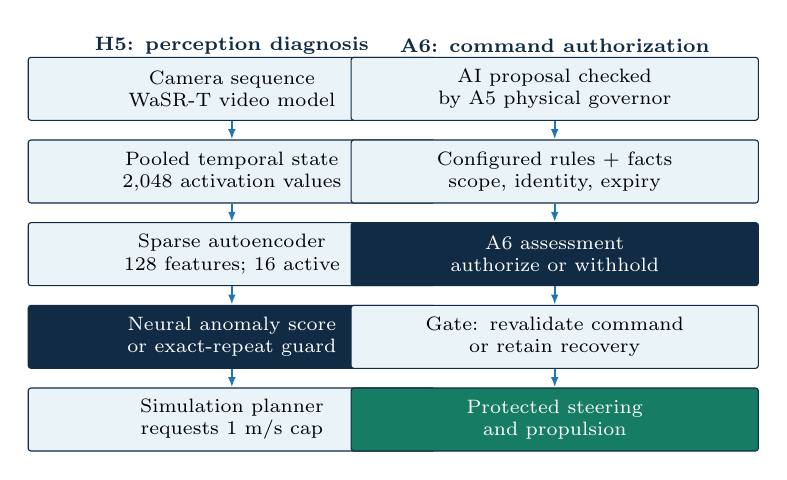
\begin{tikzpicture}[every node/.style={font=\scriptsize,align=center},
box/.style={draw=navy,rounded corners=1pt,text width=.415\columnwidth,minimum height=8mm,inner sep=2pt},
arr/.style={-{Latex[length=1.3mm]},blue,thick}]
\node[font=\scriptsize\bfseries,text=navy] at (0,0.55) {H5: perception diagnosis};
\node[font=\scriptsize\bfseries,text=navy] at (4.1,0.55) {A6: command authorization};
\node[box,fill=pale] (v) at (0,0) {Camera sequence\\WaSR-T video model};
\node[box,fill=pale] (x) at (0,-1.05) {Pooled temporal state\\2,048 activation values};
\node[box,fill=pale] (z) at (0,-2.10) {Sparse autoencoder\\128 features; 16 active};
\node[box,fill=navy,text=white] (w) at (0,-3.15) {Neural anomaly score\\or exact-repeat guard};
\node[box,fill=pale] (p) at (0,-4.20) {Simulation planner\\requests 1 m/s cap};
\node[box,fill=pale] (a) at (4.1,0) {AI proposal checked\\by A5 physical governor};
\node[box,fill=pale] (r) at (4.1,-1.05) {Configured rules + facts\\scope, identity, expiry};
\node[box,fill=navy,text=white] (d) at (4.1,-2.10) {A6 assessment\\authorize or withhold};
\node[box,fill=pale] (g) at (4.1,-3.15) {Gate: revalidate command\\or retain recovery};
\node[box,fill=green,text=white] (act) at (4.1,-4.20) {Protected steering\\and propulsion};
\draw[arr] (v)--(x);\draw[arr] (x)--(z);\draw[arr] (z)--(w);\draw[arr] (w)--(p);
\draw[arr] (a)--(r);\draw[arr] (r)--(d);\draw[arr] (d)--(g);\draw[arr] (g)--(act);
\end{tikzpicture}
\caption{Two complementary checks. H5 warnings affect the simulation planner's next proposal; that proposal still passes through A5 and the right-hand command path. A6 checks policy evidence, while the gate and watchdog retain physical recovery authority.}
\label{fig:architecture}
\end{figure}

\subsection{What ``accuracy'' means here}
Three different outcomes are measured. \textbf{Perception detection} asks whether a health warning coincides with a labelled missed-obstacle proxy. \textbf{Control assurance} measures gate acceptance, collision outcomes, and deadline behavior. \textbf{Policy enforcement} measures authorization or veto of an exact command under configured evidence. Gate acceptance is not a classifier accuracy, and a correct veto is not proof of a completed safe mission.

\callout{\textbf{Implementation choice.} A6 adds policy enforcement; H5 adds perception diagnosis. Unknown or stale evidence can preserve or reduce authority, but cannot expand it.}




\section{A-series: physical assurance and policy enforcement}
\begin{table*}[t]
\centering\small
\caption{A-series architecture family. A6 restricts the A5 command path rather than replacing the physical controller.}
\label{tab:architectures}
\begin{tabularx}{\textwidth}{@{}p{0.35in}p{2.4in}X@{}}
\toprule
\textbf{ID} & \textbf{Mechanism} & \textbf{Role in the implemented system}\\
\midrule
A1 & CPA/TCPA thresholds with Simplex switching & Transparent closest-approach baseline; the independent gate still revalidates its output.\\
A2 & Gaussian collision-risk approximation & Uncalibrated analytic risk baseline with recovery switching.\\
A3 & Finite predictive recoverability & Accepts a proposal only after checking a complete recovery continuation.\\
A4 & Plant-map barrier search and 3DOF rollout & Searches for a compatible correction, then validates its full vessel rollout.\\
A5 & Evidence-conditioned A3/A4 hybrid & Adjusts bounds and speed to health; combines predictive checking and corrective control.\\
A6 & Gate-owned command policy authorization & Restricts A5 normal commands using exact-command, evidence, and source bindings.\\
\bottomrule
\end{tabularx}
\end{table*}


The physical design combines predictive safety-filtering ideas~\cite{wabersich} with barrier-motivated correction~\cite{ames}, implemented through finite search and vessel rollouts.

\subsection{Physical-control experiment}
The original design crossed four encounter classes with three paired seeds and five candidates: 12 episode identities and 60 branches, each lasting 30 simulated seconds. Scenarios were recoverable crossing, dense traffic, vessel degradation, and initially unrecoverable encounters. All branches retained the same observation and fault identities within a pair. The profile assigned zero front-end service delay and 20\,ms each to candidate and gate service; host compute time was also recorded.

A5 preserved a 6\,m/s cap with healthy evidence, expanded bounds by 1.5 and capped speed at 3\,m/s when degraded, and forced recovery with a 1\,m/s cap when invalid. It checked the proposal plus a recovery continuation, attempted A4 correction if needed, then fell back to recovery or minimum risk.

\begin{center}
\begin{minipage}{\columnwidth}
\centering
\captionof{table}{Historical A1--A5 development comparison; 12 branches per candidate, revision \texttt{28eb923}.}
\small
\begin{tabular}{@{}lrrrr@{}}
\toprule
 & Gate & Deadline & \multicolumn{2}{c}{Compute (ms)}\\
 & accepted & misses & p50 & p95\\
\midrule
A1 & 8.87\% & 0 & 1.657 & 31.695\\
A2 & 8.73\% & 1 & 3.230 & 32.587\\
A3 & 99.66\% & 6 & 29.480 & 33.629\\
A4 & 99.44\% & 10 & 29.635 & 33.479\\
\textbf{A5} & \textbf{99.83\%} & \textbf{3} & \textbf{29.056} & \textbf{33.536}\\
\bottomrule
\end{tabular}
\end{minipage}
\end{center}

All 45 declared-recoverable branches avoided collision; all 15 initially-unrecoverable branches collided. No unsafe or stale decision was accepted. All 60 missions were incomplete at the horizon, and 40 branches exceeded an engineering uncertainty bound. The gate and watchdog contributed to these trajectories.

In the later nonzero-delay crossing experiment, A5 intervened at 0.3\,s, 39.7\,s before the sampled recovery boundary, versus 18.7\,s for A3 and 20.7\,s for A4. A5 had 183 accepted decisions and seven deadline misses. No candidate obtained gate acceptance in the out-of-domain dense-traffic case. These results motivate retaining A5 as the physical development lead.


\subsection{Policy authorization: code name A6}
A physically feasible maneuver may still lack permission under the configured operating rules. The \emph{gate-owned policy authorization layer}, called \textbf{A6}, answers: ``May this exact command be issued under the facts available now?'' It is a deterministic rule evaluator, not a learned planner or a second collision predictor. Its separation of the proposing agent from a restrictive checker resembles shielding~\cite{shielding}; Horizon checks bounded maritime rule proxies rather than synthesizing a temporal-logic shield.

A6 consumes the command checked by A5, a current snapshot of the vessel and contacts, a versioned policy bundle, and independent evidence. It first checks scope, provenance, identity, and expiry; next it evaluates supported lookout, safe-speed, collision-risk, and encounter conditions. It then emits \emph{authorize} or \emph{withhold}, with reasons and hashes binding the result to that exact command and snapshot. The gate rechecks validity before dispatch.

For example, A5 may find a 3 m/s proposal physically recoverable, yet a 1 m/s policy cap makes A6 withhold it. Missing or ambiguous facts also withhold normal authority. The gate rechecks recovery or selects minimum risk; emergency and watchdog overrides remain available.

\subsection{Maritime sources and executable rules}
The rule vocabulary follows COLREGs~\cite{colregs}. \textbf{Rule 5} becomes fresh visual, auditory, radar, and supervisor-availability evidence. \textbf{Rule 6} becomes a configured speed bound and stopping distance plus reserve within declared clear distance. \textbf{Rules 7--8} require doubt to be treated as collision risk and check action lead time, magnitude, and detectability. \textbf{Rules 13--17} classify overtaking, head-on, and crossing encounters, then check give-way or stand-on evidence; the head-on proxy requires starboard course change. Numeric margins are engineering parameters in the versioned bundle, not constants prescribed by COLREGs.

The implemented profile is a remotely supervised Singapore government USV in daylight and clear visibility. Ambiguous encounter geometry or unsupported conditions withhold normal authority. The 2026 MASS Code, resolution MSC.595(111)~\cite{mass}, provides the design-assurance reference: sections 8.3--8.4 motivate scope and fallback checks, 8.7 human supervision, and 9.10 decision logging. The bundle records MASS as a design reference and separately requires a runtime-authority source pin with revision and digest. This preserves the distinction between an architectural safety rationale and the evidence authorizing a particular command.

\subsection{Measured policy counterfactuals}
Nine five-second normal-transit branches used three seeds and three arms. Each arm generated 72 A5 pass decisions. A permissive 6\,m/s policy retained normal authority; a restrictive 1\,m/s policy replaced it with recovery.

\begin{center}
\begin{minipage}{\columnwidth}
\centering
\captionof{table}{Functional policy enforcement. The restrictive arm made three initial vetoes, one per seed; the remaining substitutions followed the recovery latch.}
\small
\begin{tabular}{@{}lrr@{}}
\toprule
Arm & Normal accepted & Recovery accepted\\
\midrule
A5 baseline & 72 & 0\\
A6 permissive & 72 & 0\\
A6 speed veto & 0 & 72\\
\bottomrule
\end{tabular}
\end{minipage}
\end{center}

All arms recorded zero collisions and trace mismatches, with 69 watchdog actions and 72 command expiries per arm. Sparse proposal cadence caused authority turnover.

The 12-episode A6 rerun accepted 1,770/1,788 A5 decisions and rejected 18 for deadline invalidity. All valid decisions used recovery or minimum risk, producing no normal policy authorizations. The nine declared-recoverable episodes remained safe in the scorer; the three initially-unrecoverable episodes did not. This design cannot measure positive-policy coverage.



\section{H-series: monitoring the video model}

\subsection{Why inspect internal representations?}
WaSR-T uses recent frames to distinguish maritime obstacles from changing water appearances~\cite{wasrt}. Its output is an obstacle/water/sky segmentation mask, and it can run independently of Horizon's monitor. Output confidence reports what the model predicts, but may remain high when a repeated image produces a stable, incorrect view of the current world. Hidden-state monitoring asks an additional question: does the model's internal processing resemble the reference behavior?

Horizon compares progressively richer signals. H0 uses output uncertainty. H1 uses conventional exposure, blur, timing, freeze, horizon, occlusion, and output-change checks. H2 measures diagonal Mahalanobis novelty in a grouped encoder summary. H3 measures PCA reconstruction error in that representation. H4 learns sparse features from the pooled image encoder. H5 moves to the temporally fused representation and explicitly trains temporal coherence.

H1's full composite lacked independent horizon and occlusion observations for evaluation. Its repeated-pixel check still complements neural monitoring.

\subsection{Temporal sparse perception monitor: H5}
The \emph{temporal sparse perception monitor}, code-named \textbf{H5}, reads WaSR-T's internal activations, learns recurring development-sequence patterns, and warns when activations reconstruct poorly or change unusually. It diagnoses processing behavior without changing the mask or producing navigable geometry.

A sparse autoencoder compresses an activation vector into a small set of active learned features and reconstructs the original vector. TopK sparsity controls how many features are used~\cite{gao}. Here a feature is a learned activation pattern, not automatically a named object such as a buoy. WaSR-T uses the current frame with up to five preceding frames. H5 spatially averages the 2,048 temporal-fusion channels, normalizes them against a pinned reference, and encodes them into 128 latent features. Hard TopK retains 16 active features per observation. A linear decoder reconstructs the normalized representation.

Writing the normalized activation as $x_t$, the sparse code as $z_t$, and reconstruction as $\hat{x}_t$, the representation warning statistic is
\[
 s_t=\operatorname{MSE}(x_t,\hat{x}_t)
       +0.1\,d(z_t,z_{t-1}),
\]
where $d(z_t,z_{t-1})=\|z_t-z_{t-1}\|_2^2/128$. Reconstruction error measures unfamiliar internal patterns; temporal distance measures changes in the sparse code. The simulation wrapper compares this statistic with the frozen simulation threshold $\tau=2.731332008015018$. The training objective separately combines reconstruction with a temporal triplet loss: adjacent frames form positive pairs and another sequence supplies the negative.

The first observation lacks a previous embedding and is unknown. The full health contract also requires conventional evidence and calibrated semantics; the simulation warning is a separate, explicitly limited response signal. It requests a 1\,m/s fixture speed cap while A5 and the gate retain final control.


\subsection{Training and causal feature evidence}
Eight development sequences from \texttt{kope81} supplied 40 uniformly sampled frames each. Five sequences fitted candidate configurations and three measured validation reconstruction and temporal separation. A fixed grid varied feature count, sparsity, and temporal weight. Eligible models had to converge, retain at least 90\% live features, and reconstruct within 10\% of the best eligible error; selection then favored temporal separation.

The selected configuration was refitted with seeds 0, 1, and 2. Its 320-frame fit converged in 622 epochs with 3/128 dead features. Relative to a capacity-matched zero-temporal-weight model:

\begin{center}
\begin{minipage}{\columnwidth}
\centering
\captionof{table}{Temporal training improved reconstruction and code separation on development validation sequences.}
\small
\begin{tabularx}{\columnwidth}{@{}Xrr@{}}
\toprule
Measure & No temporal loss & H5\\
\midrule
Validation MSE & 0.9533 & 0.8295\\
Cross/adjacent distance ratio & 6.12 & 6.89\\
\bottomrule
\end{tabularx}
\end{minipage}
\end{center}

Reconstruction alone does not establish that a feature matters to the output. Following the causal-intervention perspective of sparse feature circuits~\cite{marks}, we intervene on a selected direction and compare its effect with matched controls. Whole-dictionary reproducibility remained weak: mean nearest decoder cosine was 0.425. The selected feature 55 passed the feature-specific gate, with minimum decoder cosine 0.528 and activation correlation 0.667 across alternate seeds. Its layer intervention exceeded both random-direction and equal-norm controls in 18/18 trials across three probe sequences and three seeds. H4's validated direction won 15/18 trials. These are causal-feature comparisons, not percentages of camera failures detected.

\subsection{Sustained-freeze guard}
The neural representation can stay stable during a frozen feed. Horizon therefore adds a separate exact-RGB repeat check to the H5 simulation wrapper. Three consecutive duplicate observations trigger \texttt{frozen\_feed}: four identical images including the original. Changed pixels clear the counter, while stale, missing, out-of-order, expired, or sequence-mismatched evidence resets it. The combined warning fires on either the neural threshold or the repeat guard.

\callout{\textbf{Independent evidence.} Neural novelty detects some representation failures; the repeat guard detects sustained exact freezes. The guard changes neither WaSR-T weights nor H5 training. Near-duplicate images require a different detector, and total feed loss is handled through freshness checks.}




\section{Experiment execution and L4 latency}

\subsection{NVIDIA L4 execution protocol}
The recorded CUDA job processed all 296 left-camera frames of \texttt{kope81-00-00006800-}\allowbreak\texttt{00007095}. Its Modal container used one NVIDIA L4, four CPU cores, 16\,GiB host memory, no retries, and a 1,200\,s cap. The runner verified frame count, input bytes, and the frozen split hash.

The environment was Python 3.11.12, PyTorch 2.5.1+cu124, torchvision 0.20.1+cu124, CUDA 12.4, cuDNN 90100, and Pillow 10.4.0. WaSR-T's ResNet101 temporal model used upstream commit \texttt{1b5360af2040} and checkpoint digest \texttt{6e70dd6583a9}. The manifest retains the complete hashes. CUDA inference used FP16; the matched Apple M1 Max MPS arm used FP32.

Images were decoded to RGB, resized to $512\times384$ pixels with antialiased interpolation, normalized with ImageNet channel statistics, and processed sequentially at batch size one. Temporal state was reset at sequence boundaries. The runner captured encoder, temporal-fusion, and decoder-logit summaries, raw class masks, color previews, and fixed spatial probes at five positions.

Before extraction, vanilla and instrumented inference received the same one-frame warm-up and three measured frames. Logits matched exactly, and state reset reproduced the outputs exactly within each backend. The L4 comparison measured 33.203\,ms mean vanilla and 36.349\,ms instrumented forward time, a 3.146\,ms difference in this three-frame check.

\subsection{What the timers include}
The forward timer synchronizes CUDA or MPS immediately before and after the model call. It includes activation-hook work but excludes image decode, preprocessing, model load, and subsequent CPU stages. A separate timer measures output transfer, another measures CPU resizing, and another measures output-health and conventional-feature extraction. Hook-capture time overlaps the forward timer and must not be added again.

For each cached frame we derived a recorded compute subtotal:
\[
T_{\mathrm{sub}}=T_{\mathrm{forward}}+T_{\mathrm{copy}}
                 +T_{\mathrm{resize}}+T_{\mathrm{health}}.
\]
Its quantiles below use per-frame sums, not sums of quantiles. Linear interpolation defines p95; all recorded sequence frames are retained. The subtotal excludes file writing, publication, H5 SAE scoring, fusion, policy, and actuation.


\subsection{Recorded timing results}
\begin{center}
\begin{minipage}{\columnwidth}
\centering
\captionof{table}{Milliseconds from archived frame records. Quantiles and subtotals are recalculated from existing logs; no new inference was run for this paper.}
\small
\begin{tabular}{@{}lrrr@{}}
\toprule
Stage / runtime & p50 & p95 & Max\\
\midrule
\multicolumn{4}{@{}l}{\textbf{L4 FP16, 296 development frames}}\\
Forward & 34.91 & 37.07 & 40.36\\
CPU health & 108.31 & 125.91 & 141.47\\
Compute subtotal & 144.75 & 162.92 & 185.36\\
\addlinespace
\multicolumn{4}{@{}l}{\textbf{MPS FP32, same 296 inputs}}\\
Forward & 799.92 & 819.50 & 839.92\\
CPU health & 75.37 & 91.32 & 104.34\\
Compute subtotal & 877.39 & 903.18 & 936.47\\
\bottomrule
\end{tabular}
\end{minipage}
\end{center}

The 296-frame forward medians differ by a factor of 22.9, whereas the recorded compute subtotals differ by 6.1. These are descriptive cross-host and cross-precision ratios. CPU health extraction dominates the L4 subtotal, making it the first optimization target. A 34.91\,ms model call fits within 50\,ms, but the measured pipeline subtotal does not establish 20\,Hz end-to-end operation.

The same-input backend comparison found p95 relative representation differences of 0.003637 in the encoder, 0.009944 in temporal fusion, and 0.002857 in decoder logits. Mask disagreement was 0.01742\% of pixels at p95. This measures runtime agreement, not segmentation accuracy. Thresholds fitted on MPS therefore require validation on the intended CUDA execution path.




\subsection{Control and policy timing}
A5's historical p50/p95 compute was 29.056/33.536\,ms. The earlier A6 shadow evaluated 1,788 decisions at 0.178/0.281\,ms p50/p95, with a 0.394\,ms maximum. That measures the shadow evaluator, not the current complete authorization and dispatch path. Enforcement checks a 10\,ms policy budget after evaluation; the budget is not a measured latency or preemptive timeout.

The controller studies, MPS accuracy studies, and L4 extraction jobs are distinct experiments. Their stage times cannot be summed into a measured sensor-to-actuator latency. Synthetic 10\,Hz image timestamps preserve frame order only; they do not demonstrate live throughput.



\begin{figure*}[t]
\centering
\begin{tikzpicture}
\begin{groupplot}[group style={group size=2 by 1,horizontal sep=1.4cm},
 width=.46\textwidth,height=4.6cm,xmin=0,xmax=1,
 tick label style={font=\scriptsize},label style={font=\small},
 title style={font=\small\bfseries},grid=major,grid style={gray!15},
 legend style={font=\scriptsize,draw=none,fill=white},no markers]
\nextgroupplot[title={ROC: ranking across thresholds},xlabel={False-positive rate},ylabel={Recall},ymin=0,ymax=1,legend pos=south east]
\addplot[blue,thick] table[x=x,y=y,col sep=comma]{figures/h0-roc.csv};\addlegendentry{H0: 0.664}
\addplot[orange!85!black,dashed,thick] table[x=x,y=y,col sep=comma]{figures/h2-roc.csv};\addlegendentry{H2: 0.639}
\addplot[violet,densely dotted,thick] table[x=x,y=y,col sep=comma]{figures/h3-roc.csv};\addlegendentry{H3: 0.521}
\addplot[gray!70!black,dashdotted,thick] table[x=x,y=y,col sep=comma]{figures/h4-roc.csv};\addlegendentry{H4: 0.641}
\addplot[green,very thick] table[x=x,y=y,col sep=comma]{figures/h5-roc.csv};\addlegendentry{H5: 0.712}
\addplot[black!45,dashed,forget plot] coordinates {(0,0) (1,1)};
\addplot[only marks,mark=*,mark size=2pt,black,forget plot] coordinates {(0.01915252555324005,0.21212121212121213)};
\nextgroupplot[title={PR: reliability of warnings},xlabel={Recall},ylabel={Precision (log scale)},ymode=log,ymin=.001,ymax=1,legend pos=north east,unbounded coords=jump]
\addplot[blue,thick] table[x=x,y=y,col sep=comma]{figures/h0-pr.csv};\addlegendentry{H0: 0.0103}
\addplot[orange!85!black,dashed,thick] table[x=x,y=y,col sep=comma]{figures/h2-pr.csv};\addlegendentry{H2: 0.0043}
\addplot[violet,densely dotted,thick] table[x=x,y=y,col sep=comma]{figures/h3-pr.csv};\addlegendentry{H3: 0.0036}
\addplot[gray!70!black,dashdotted,thick] table[x=x,y=y,col sep=comma]{figures/h4-pr.csv};\addlegendentry{H4: 0.0066}
\addplot[green,very thick] table[x=x,y=y,col sep=comma]{figures/h5-pr.csv};\addlegendentry{H5: 0.0515}
\addplot[black!45,dashed,forget plot] coordinates {(0,.003264094955489614) (1,.003264094955489614)};
\addplot[only marks,mark=*,mark size=2pt,black,forget plot] coordinates {(0.21212121212121213,.035)};
\end{groupplot}
\end{tikzpicture}
\caption{ROC and precision--recall from 10,110 matched MPS records (33 positives). Legends report AUROC (left) and average precision (right). Dashed reference lines show chance ranking and positive prevalence; black dots mark the frozen H5 operating point. PR uses logarithmic precision to expose behavior at this rare-event rate; zero-precision points are outside that axis. No inference or threshold refitting was performed.}
\label{fig:curves}
\end{figure*}

\begin{table*}[t]
\centering\small
\caption{Matched missed-obstacle proxy results. AP is average precision. H1 was excluded because its required independent signals were unavailable. The common false-positive ceiling was applied during threshold selection; realized evaluation FPR differs by method.}
\begin{tabularx}{\textwidth}{@{}Xrrrrrrrr@{}}
\toprule
Method & Accuracy & Balanced & Precision & Recall & F1 & FPR & AUROC & AP\\
\midrule
H0 & 97.95\% & 53.67\% & 1.67\% & 9.09\% & 2.82\% & 1.76\% & 0.664 & 0.0103\\
H2 & 91.60\% & 45.95\% & 0.00\% & 0.00\% & 0.00\% & 8.10\% & 0.639 & 0.0043\\
H3 & 92.17\% & 47.74\% & 0.13\% & 3.03\% & 0.25\% & 7.54\% & 0.521 & 0.0036\\
H4 & 98.94\% & 49.63\% & 0.00\% & 0.00\% & 0.00\% & 0.73\% & 0.641 & 0.0066\\
\textbf{H5} & \textbf{97.83\%} & \textbf{59.65\%} & \textbf{3.50\%} & \textbf{21.21\%} & \textbf{6.01\%} & \textbf{1.92\%} & \textbf{0.712} & \textbf{0.0515}\\
\bottomrule
\end{tabularx}
\end{table*}

\section{Detection accuracy and fault coverage}

\subsection{Scoring protocol}
H2--H5 references were fitted on \texttt{kope81}. The \texttt{kope67} calibration group selected one threshold per method by maximizing recall under a 5\% empirical false-positive ceiling. The frozen thresholds were then applied to four sequences from the disjoint \texttt{kope75} collection. Each sequence had nominal, blur, underexposure, occlusion, JPEG, and temporal-drop arms.

All methods used the same 10,110 frames after excluding the first frame of each sequence/arm for temporal context. These acquisitions ran on MPS FP32. The sealed \texttt{kope71}/\texttt{kope82} groups were not used. Predictions were compared with a fixed bounding-box proxy: a positive frame contains at least one annotated obstacle box with zero predicted obstacle pixels. This is a missed-obstacle proxy, not official MODD2 segmentation accuracy.


\subsection{Class imbalance and interpretation}
Only 33 frames were positive and 10,077 were negative. An always-negative detector would achieve 99.67\% accuracy while detecting no misses. We therefore report recall, precision, balanced accuracy, false-positive rate, and ranking quality together:
\[
\mathrm{Recall}=\frac{TP}{TP+FN},\qquad
\mathrm{Precision}=\frac{TP}{TP+FP},
\]
\[
\mathrm{Balanced\ accuracy}=\tfrac12(\mathrm{Recall}+\mathrm{Specificity}).
\]
Adjacent frames are dependent; these results describe the evaluated collection shift and fault arms.

\subsection{ROC and precision--recall across thresholds}
Receiver operating characteristic (ROC) curves plot recall against false-positive rate as the warning threshold varies; AUROC summarizes score ranking~\cite{fawcett}. They are appropriate for H0 and H2--H5 because each returns a continuous score. A6 returns a rule-based authorization decision, so it has no corresponding score sweep in these experiments.

With only 0.326\% positives, precision--recall (PR) is an essential companion: it shows what fraction of warnings identify a proxy miss~\cite{saito}. Figure~\ref{fig:curves} is reconstructed from the same hash-verified cached activations and labels, with equal scores grouped. AP weights threshold precision by each increase in recall. The original thresholds are unchanged. H5's AUROC of 0.712 and AP of 0.0515 lead the comparison, but its operating point remains 21.21\% recall and 3.50\% precision. The curves cover neural scores; they are not a combined A6/H5 or freeze-guard accuracy measure.


\vspace{-3pt}


\subsection{Where H5 helped}
H5 produced $TP=7$, $FN=26$, $FP=193$, and $TN=9{,}884$. It had the highest AUROC, AP, recall, and balanced accuracy among the executable monitors. H0, which uses model output uncertainty, detected 3/33 misses; H5 detected 7/33. This is a count comparison and does not imply disjoint detections or a calibrated failure probability.

All seven H5 detections were in occlusion: 7/16 misses. It detected 0/1 nominal, 0/1 blur, 0/4 underexposure, 0/1 JPEG, and 0/10 temporal-drop misses. The 193 false warnings also occurred in occlusion. Thus H5's present advantage is concentrated in this arm, with low precision and incomplete coverage.

The subsequent freeze-guard rerun processed 10,134 frames through the current wrapper using hash-verified cached activations and decoded images. Excluding the 24 context-initialization frames reproduced the original confusion matrix exactly. All 337 duplicate frames were isolated repeats; none reached the three-repeat trigger. The guard added no detections and no false positives on this dataset.





\subsection{Controlled blackout and freeze}
The real-model MPS test used one 60-frame clip in three arms: original video, blackout, and freeze. Fault arms contained 20 normal, 20 fault, and 20 recovery frames. All 180 input hashes and neural scores matched the guard-enabled rerun.

\begin{center}
\begin{minipage}{\columnwidth}
\centering
\captionof{table}{Fault-window warning coverage; one episode per injected fault, with one initial unknown frame in each arm.}
\small
\begin{tabular}{@{}lrr@{}}
\toprule
Window & Neural only & With guard\\
\midrule
Blackout (20 frames) & 20/20 & 20/20\\
Freeze (20 frames) & 0/20 & 18/20\\
Original clip (60 frames) & 0 warnings & 0 warnings\\
\bottomrule
\end{tabular}
\end{minipage}
\end{center}

The blackout warning began on the first black frame and cleared after three recovery frames. The freeze guard began on the third repeated observation and cleared on the first changed image. Freeze coverage was therefore 90\% of fault frames after intentional debounce, not 90\% event-level detection accuracy. The neural freeze score remained only 0.047--0.060.

Simple darkness and duplicate checks cover these injections. Detection delays are in frames, not measured live elapsed time.



\section{System integration and the A6 + H5 decision}

\subsection{Did warnings change decisions?}
The warning-response study paired two scenarios, two video arms, three seeds, and H5 off/on: 24 episodes. Transit lasted 100\,s and crossing 120\,s. Both branches shared A5, radar, planner, and gate, with A6 disabled to isolate the response. Hash-pinned H5 tapes supplied warnings without live video inference.

In occluded-video normal transit, enabling H5 produced 39 warning requests per run, all accepted as autonomy commands at or below 1\,m/s. Mean distance travelled changed from 46.28 to 45.31\,m. In crossing, 59 warning requests per run yielded no accepted slow autonomy commands because the gate retained recovery authority. Mean minimum hull clearance changed from 146.09 to 145.98\,m. These observations verify both the response path and the gate's ability to retain control.

All 24 episodes had zero collisions, zero arrivals, complete traces, and zero authority-trace mismatches. No collision reduction or arrival-time benefit was observed. The consumed warning windows were proxy-negative: 7.8\,s of warning requests per transit run and 11.8\,s per crossing run. Recorded video did not depict the simulated encounters, so clearance changes cannot be attributed to recognition of the simulated hazards.


\subsection{Implementation priorities}
Priorities are CPU health optimization, complete publication-to-command timing, CUDA threshold validation, and sealed-group evaluation with sequence-level uncertainty. Pose-reactive video and completed journeys would measure navigation benefit.

\subsection{Conclusion: why A6 with H5}
\textbf{We choose to implement A6 with H5 around A5 because the three components address different failure sources.} A5 supplies evidence-conditioned physical checking and recovery. Its 99.83\% historical gate acceptance and early crossing intervention support retaining it as the physical development controller. A6 then restricts normal authority to commands supported by exact, current policy evidence; the counterfactual test shows 72 normal commands retained under a permissive policy and zero under the restrictive policy.

H5 contributes the strongest measured proxy-miss ranking in the evaluated H-series: AUROC 0.712 and 7/33 misses detected. Its temporal feature has stronger development causal-control results than the tested H4 direction, and the separate repeat guard supplies sustained-freeze coverage that neural novelty alone missed. Keeping these diagnostics separate preserves clear explanations for each warning.

The design reduces simulated speed on warnings, withholds policy-incompatible commands, and preserves recovery under uncertainty. Complementary measured capabilities motivate this engineering selection; broader coverage and integrated target-hardware trials are the next tests.


\begin{thebibliography}{10}
\footnotesize
\bibitem{shielding} Mohammed Alshiekh, Roderick Bloem, R\"udiger Ehlers, Bettina K\"onighofer, Scott Niekum, and Ufuk Topcu. 2018. Safe Reinforcement Learning via Shielding. In \emph{Proceedings of the AAAI Conference on Artificial Intelligence} 32(1). \url{https://doi.org/10.1609/aaai.v32i1.11797}
\bibitem{ames} Aaron D. Ames, Xiangru Xu, Jessy W. Grizzle, and Paulo Tabuada. 2017. Control Barrier Function Based Quadratic Programs for Safety Critical Systems. \emph{IEEE Transactions on Automatic Control} 62(8), 3861--3876. \url{https://doi.org/10.1109/TAC.2016.2638961}
\bibitem{fawcett} Tom Fawcett. 2006. An introduction to ROC analysis. \emph{Pattern Recognition Letters} 27(8), 861--874. \url{https://doi.org/10.1016/j.patrec.2005.10.010}
\bibitem{gao} Leo Gao, Tom Dupr\'e la Tour, Henk Tillman, Gabriel Goh, Rajan Troll, Alec Radford, Ilya Sutskever, Jan Leike, and Jeffrey Wu. 2024. Scaling and evaluating sparse autoencoders. \emph{arXiv:2406.04093}. \url{https://arxiv.org/abs/2406.04093}
\bibitem{colregs} International Maritime Organization. 1972. \emph{Convention on the International Regulations for Preventing Collisions at Sea (COLREGs), as amended}. Rules 5--8 and 13--17. \url{https://www.imo.org/en/about/conventions/pages/colreg.aspx}
\bibitem{mass} International Maritime Organization. 2026. \emph{International Code of Safety for Maritime Autonomous Surface Ships (MASS Code)}. Resolution MSC.595(111), non-mandatory code, sections 8.3--8.4, 8.7, and 9.10. \href{https://wwwcdn.imo.org/localresources/en/MediaCentre/Documents/MSC\%20111-22-Annex\%2016\%20(Secretariat).pdf}{MSC 111/22, Annex 16}.
\bibitem{marks} Samuel Marks, Can Rager, Eric J. Michaud, Yonatan Belinkov, David Bau, and Aaron Mueller. 2024. Sparse Feature Circuits: Discovering and Editing Interpretable Causal Graphs in Language Models. \emph{arXiv:2403.19647}. \url{https://arxiv.org/abs/2403.19647}
\bibitem{saito} Takaya Saito and Marc Rehmsmeier. 2015. The Precision-Recall Plot Is More Informative than the ROC Plot When Evaluating Binary Classifiers on Imbalanced Datasets. \emph{PLOS ONE} 10(3), e0118432. \url{https://doi.org/10.1371/journal.pone.0118432}
\bibitem{wabersich} Kim P. Wabersich and Melanie N. Zeilinger. 2021. A predictive safety filter for learning-based control of constrained nonlinear dynamical systems. \emph{Automatica} 129, 109597. \url{https://doi.org/10.1016/j.automatica.2021.109597}
\bibitem{wasrt} Lojze \v{Z}ust and Matej Kristan. 2022. Temporal Context for Robust Maritime Obstacle Detection. \emph{arXiv:2203.05352}. \url{https://arxiv.org/abs/2203.05352}
\end{thebibliography}
\end{document}
